\section{Results: Costing the Reform Menu}
\label{sec:results}

This section reports the policy payoff of the microsimulation. The headline
deliverable is a \emph{menu} of registration-threshold reforms---raising the
threshold (a \emph{location} move), a graduated \emph{taper}, and a banded
\emph{reduced rate}---costed on a common static basis and then \emph{ranked by
efficiency}: how much of the notch's distortion each reform removes relative to
its fiscal cost. The efficiency ranking (Table~\ref{tab:efficiency}) is the
paper's central policy result, and it rests on a robust, analytic object---the
notch's dominated region---rather than on any fragile simulation. I build to it
in stages: a short consistency check of the static method against HMRC's costing
of the April~2024 reform; a static sweep of threshold locations; the modest,
localised behavioural response from the calibrated model; the graduated taper;
the reduced rate; and the efficiency ranking that orders the menu.

\subsubsection{Counterfactual policy reforms}
\label{sec:counterfactuals}

This paper delivers two kinds of counterfactual. The first kind is a change to
the \emph{location} of the single VAT registration threshold. I organise these
around two objects. The first is the \emph{anchor reform}: the actual increase of
the registration threshold from \pounds85{,}000 to \pounds90{,}000 that took
effect on 1~April 2024. This is a real, recent policy change, and I benchmark my
static costing of it directly against HM Revenue and Customs' own published
costing (Section~\ref{sec:results}). The second is a \emph{forward-looking sweep}
of alternative threshold locations spanning \pounds70{,}000 to \pounds120{,}000,
costed from the post-reform \pounds90{,}000 baseline. The anchor reform tells me
whether the model reproduces a costing I can check; the sweep then maps out the
fiscal menu of further location moves.

The second kind is a change to the \emph{shape} of the schedule:
Section~\ref{sec:cf_taper} delivers a \emph{graduated taper} that replaces the
\pounds85{,}000 notch with an effective rate that phases linearly from $0\%$ at
\pounds85{,}000 to the full $20\%$ at \pounds105{,}000. A schedule-shape change has
no single point of excess mass that a reduced-form bunching estimator can
forward-map; pricing it requires re-solving each firm's choice under a new,
continuous tax function, which the calibrated model lets me do.

Alongside these threshold-location reforms, the microsimulation assigns each firm a
cost parameter $\{A_i\}$ consistent with its observed turnover and inputs
(Section~\ref{sec:model}); I make no claim to identify it as a structural
primitive. Holding $\{A_i\}$ fixed, I replace the tax schedule $\tau(\cdot)$ with a
counterfactual policy, re-solve each firm's choice for a new optimal turnover
$y_i^{\text{new}}$, and re-aggregate the weighted choices into a counterfactual
turnover distribution.

\subsubsection{What the calibrated model adds}
\label{sec:cf_valueadded}

For the revenue cost of a pure threshold-\emph{location} change, a static
mechanical calculation already captures the first-order fiscal effect---the close
HMRC consistency check in Section~\ref{sec:results} comes from that
calculation---so I do not lean on the calibrated model there. Its distinctive
payoff is to price the reform a reduced-form estimator cannot: a change to the
\emph{shape} of the schedule, which has no single point of excess mass to
forward-map. I exploit this in Section~\ref{sec:cf_taper} to replace the notch
with a graduated taper. Along the way the model also simulates the full firm-size
\emph{distribution} under unobserved thresholds and separates optimisation from
frictions, neither of which the reduced form isolates. I exploit it again for a
second schedule-shape reform---a banded reduced rate for small firms
(Section~\ref{sec:results_rate}). A \emph{sector-specific} split rate for
labour-intensive services is feasible with the same machinery but is left to future
work (Section~\ref{sec:conclusion}).

\subsubsection{Frictions matter: a dynamic re-optimisation check}
\label{sec:cf_dynamic}

Before pricing the taper, I verify that the calibrated behavioural rule, not
frictionless optimisation, is the right tool---evidence that disciplines the
model. I re-solve the firm-size distribution under a threshold move
(\pounds85{,}000 to \pounds95{,}000) under two assumptions. In the
\emph{Pure-FOC} variant every firm re-optimises fully to its new FOC solution,
collapsing the old mass and re-forming it as a sharp double spike at the new
cutoff. The \emph{FOC+Uncertainty} variant adds a threshold-aware perturbation,
$y^{\text{unc}}_i = y^{\text{FOC}}_i\,(1+\varepsilon_i)$ with
$\varepsilon_i \sim \mathcal{N}(0, \sigma_\varepsilon^{2})$,
$\sigma_\varepsilon = 0.04$, capturing the frictions and imperfect foresight that
keep firms off the kink; this replaces the double spike with a rounded hump and
reproduces the observed pattern that only a minority reposition. The frictionless
variant materially overstates the response---the quantitative gap (mean turnover
\pounds1{,}488k versus actual \pounds1{,}130k) is stated in
Section~\ref{sec:results_structural}---so FOC+Uncertainty is the variant I carry
into the taper. Figure~\ref{fig:foc_dynamic} contrasts the two against the actual
distribution.

\begin{figure}[htbp]
\centering
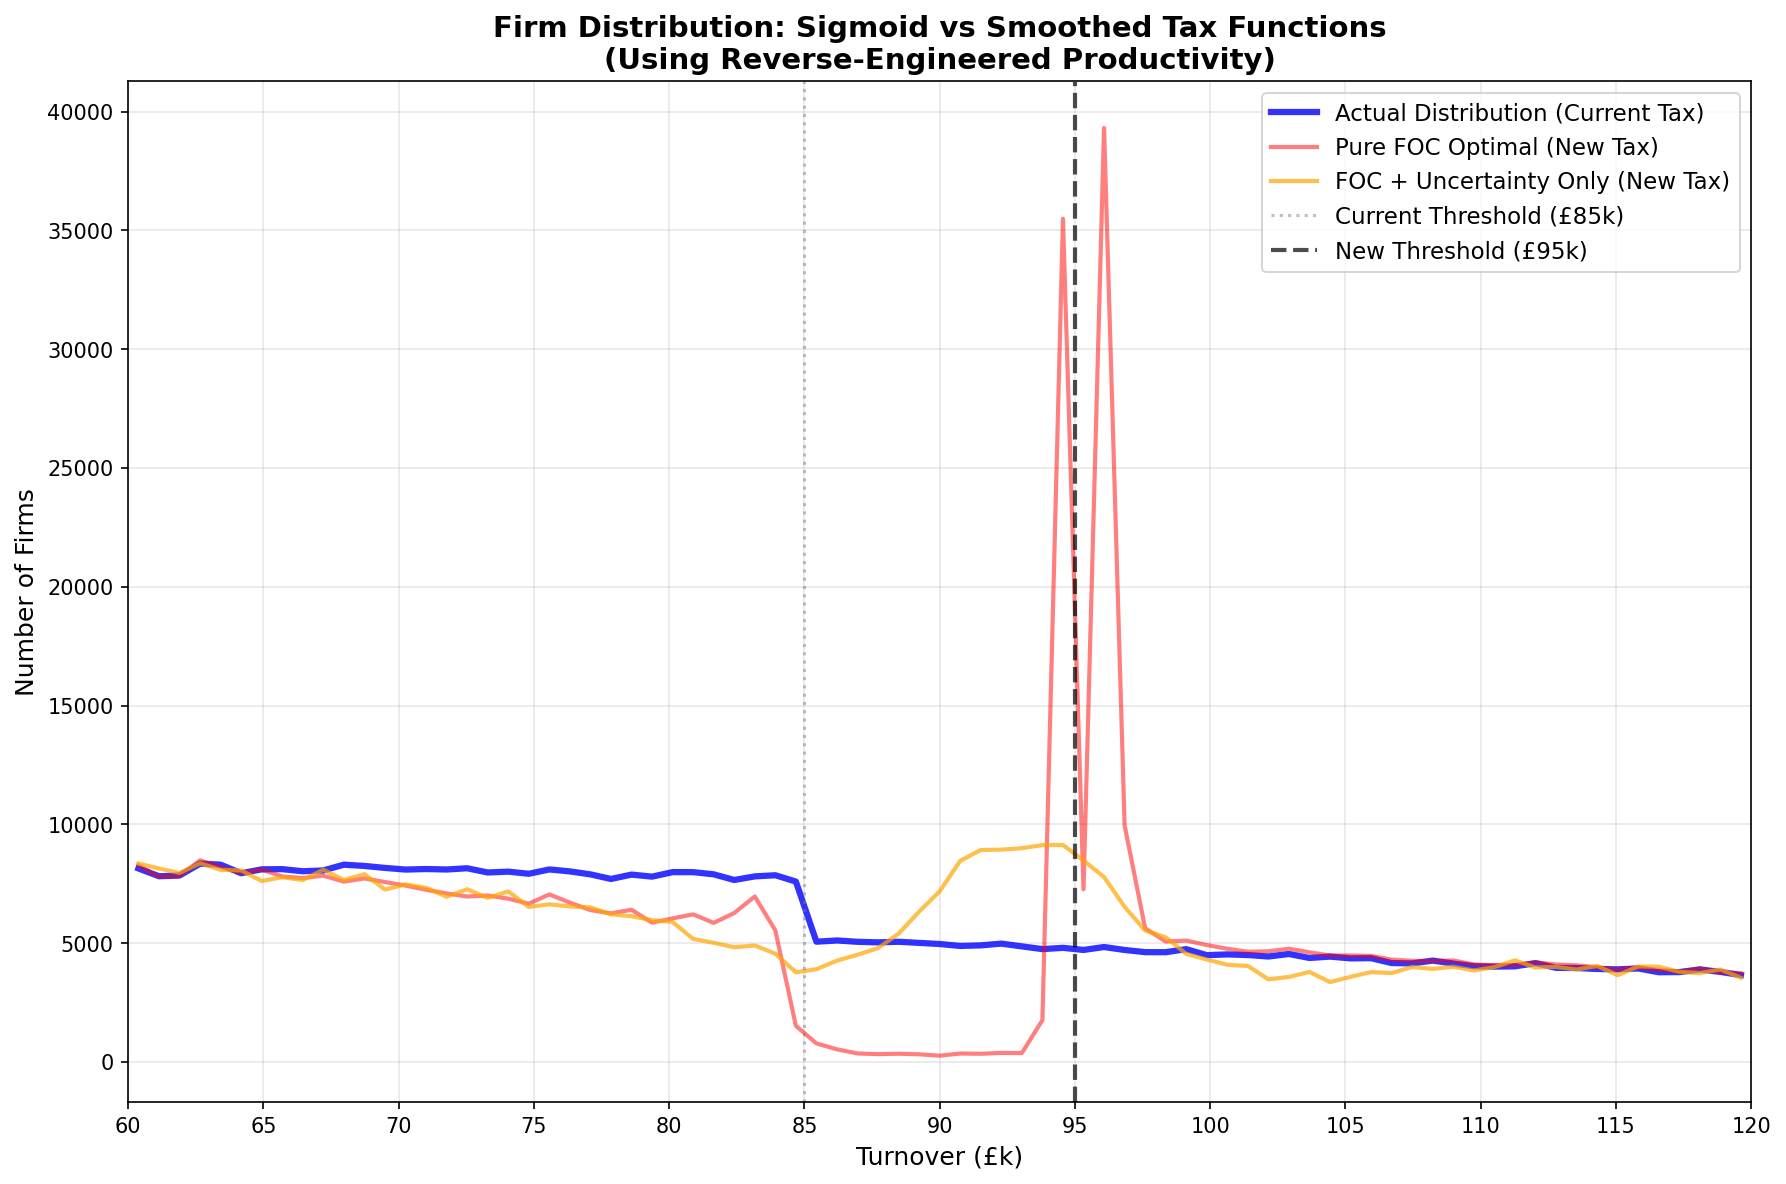
\includegraphics[width=0.9\textwidth]{figures/foc_dynamic_85kdata_full.png}
\caption{Dynamic re-optimisation under a new \pounds95{,}000 threshold, applied
to the \pounds85{,}000-era data. The \emph{Actual} distribution shows the
density step at the old \pounds85{,}000 threshold. The \emph{Pure-FOC} variant,
in which every firm re-optimises fully and frictionlessly, collapses the old mass
and re-forms it as a sharp double spike at the new \pounds95{,}000 threshold,
overstating the realised response. The \emph{FOC+Uncertainty} variant adds a
threshold-aware perturbation $\varepsilon \sim \mathcal{N}(0, 0.04^{2})$,
replacing the double spike with a smoothed hump around the new threshold that
matches the realised, partial nature of firm responses.}
\label{fig:foc_dynamic}
\end{figure}

\subsubsection{A graduated taper: the delivered schedule-shape reform}
\label{sec:cf_taper}

The dynamic experiment above still concerns a threshold-\emph{location} move,
for which the reduced form is a sufficient tool. I now use the calibrated model
for the task it alone can perform: pricing a change to the \emph{shape} of the
schedule. I replace the notch with a \emph{graduated taper}. Let $T_{0}$ denote the lower
edge of the taper band (the current registration threshold), $T_{1}$ its upper
edge, and $\tau_{\max}$ the standard VAT rate. Under the taper a firm with
turnover $y$ faces an effective rate
\begin{equation}
\tau_{\text{eff}}(y) =
\begin{cases}
0, & y < T_{0},\\[2pt]
\tau_{\max}\,\dfrac{y - T_{0}}{T_{1} - T_{0}}, & T_{0} \le y \le T_{1},\\[6pt]
\tau_{\max}, & y > T_{1},
\end{cases}
\label{eq:taper}
\end{equation}
so the effective liability phases linearly from $0$ at $T_{0}$ to the full rate
$\tau_{\max}$ at $T_{1}$. I implement the taper with $T_{0}=\pounds85{,}000$,
$T_{1}=\pounds105{,}000$ (a \pounds20{,}000 band) and $\tau_{\max}=0.20$. The taper eliminates the discrete jump in tax
liability that creates the notch: a firm that crosses \pounds85{,}000 no longer
faces VAT on its entire value added at once, only on the marginal slice implied by
its position in the band.

To price this reform I hold the calibrated firm cost parameters $\{A_i\}$ fixed
and re-optimise each firm's profit under the tapered $\tau(\cdot)$. Because
near-constant returns make the unconstrained optimum a knife edge, I re-optimise
over a bounded neighbourhood of each firm's observed turnover, consistent with the
partial, localised responses documented in Section~\ref{sec:results_structural}. The
crucial difference between the two schedules is the
\emph{local tax wedge} $y\,\tau'(y)$: under the notch this wedge is large and
concentrated at \pounds85{,}000 (it is what drives firms to bunch just below);
under the taper it is small and constant across the band, so the incentive to
suppress turnover largely disappears. The reduced-form bunching estimator cannot
evaluate this reform, because once the notch is replaced by a smooth schedule
there is no single point of excess mass to forward-map.

The quantitative results, distributional effect, and figure for the taper are
reported in Section~\ref{sec:results_taper}.

\subsubsection{Static versus behavioural evaluation}
\label{sec:cf_static_vs_behavioural}

I distinguish the dynamic, behavioural simulation above from a \emph{static}
counterpart. In the static approach, firm turnover is held fixed and the new
schedule applied mechanically, so revenue changes reflect only reclassification
across the threshold; this benchmark underlies both the anchor-reform check and
the threshold sweep. The behavioural FOC+Uncertainty simulation instead captures
the second-order offset from re-optimisation and is the relevant object for how a
reform reshapes the firm-size distribution. The revenue, firm-count, and
distributional results for the threshold-location reforms are reported in
Section~\ref{sec:results}.


\subsection{A sanity check against HMRC costings}
\label{sec:results_validation}

As a first sanity check on the static pipeline, I confirm that it reproduces HM
Revenue and Customs' own costing of the April~2024
\pounds85{,}000 to \pounds90{,}000 increase. This is a \emph{sanity
check}, not a validation: my microdata are calibrated to HMRC VAT aggregates
(Section~\ref{sec:data}), so a close match confirms only that the microdata and
revenue calculation are internally aligned with the official tax base.
Figure~\ref{fig:hmrc_validation} shows the two series share sign and profile
throughout: in 2025--26 I estimate \(-\)\pounds184m against HMRC's
\(-\)\pounds185m, and by 2028--29 both turn positive (\(+\)\pounds72m versus
\(+\)\pounds65m) as fiscal drag lifts the frozen baseline above the reformed
threshold, the largest gap being \pounds33m in 2024--25.

\begin{figure}[htbp]
\centering
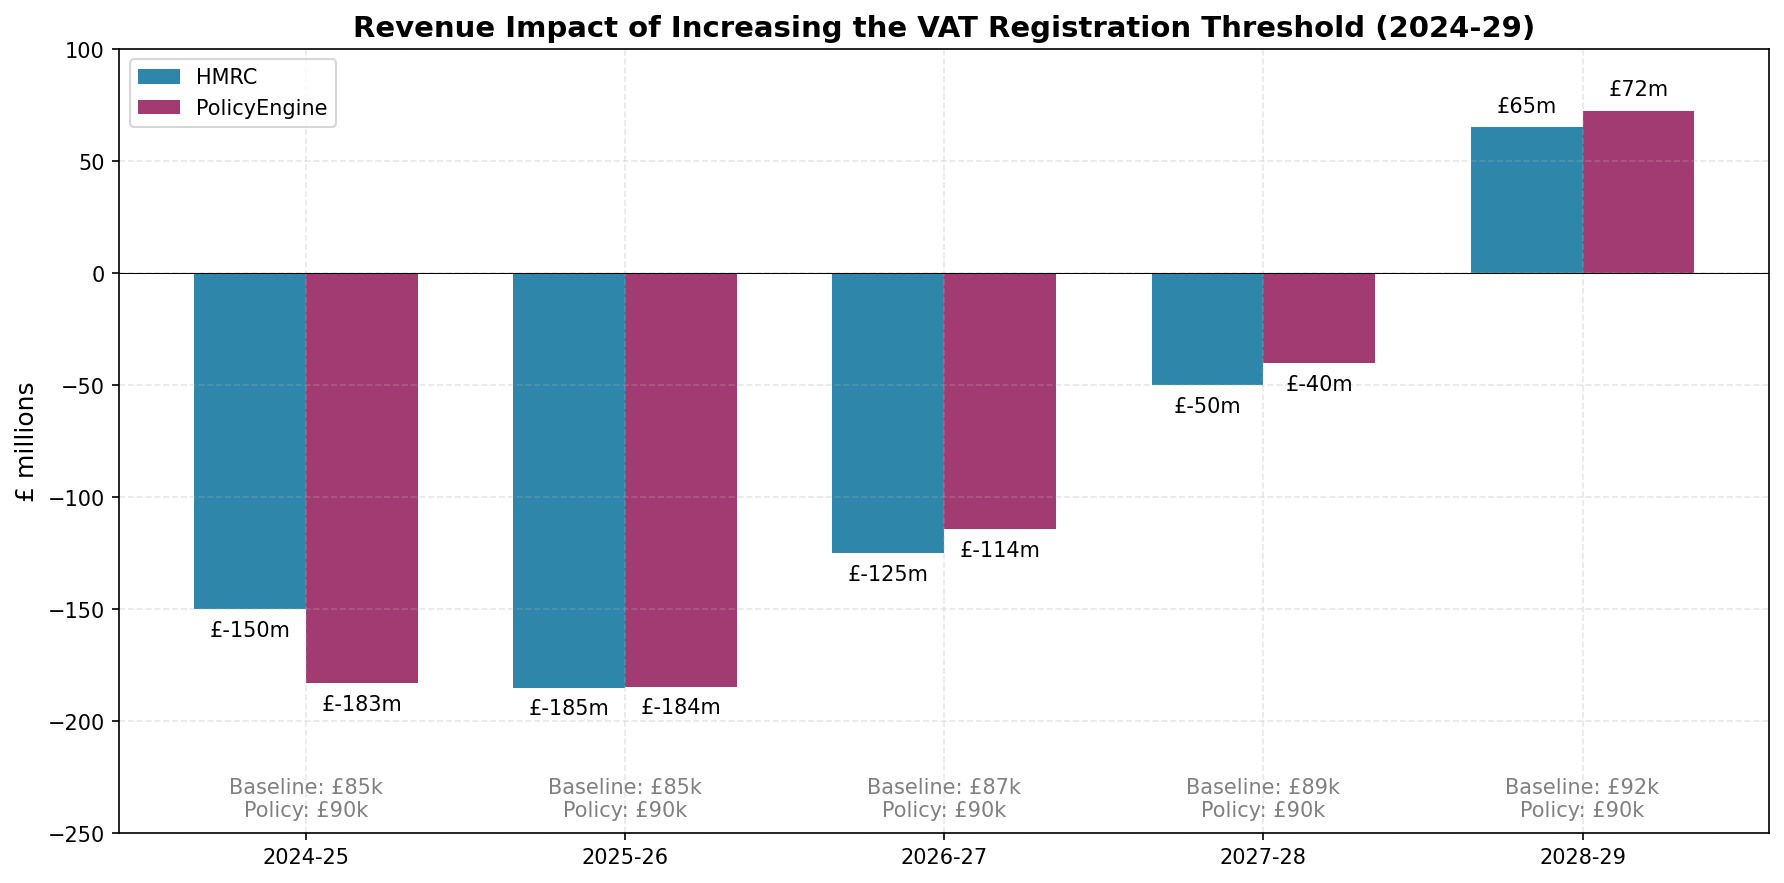
\includegraphics[width=0.92\textwidth]{figures/vat_threshold_revenue_impact.png}
\caption{Anchor reform: revenue impact of raising the VAT registration threshold
from \pounds85{,}000 to \pounds90{,}000 (the actual April~2024 change), my
estimate (PolicyEngine) versus HMRC's published costing, 2024--25 to 2028--29.
Year-by-year (PolicyEngine vs HMRC, \pounds m): 2024--25 \(-\)183 vs \(-\)150;
2025--26 \(-\)184 vs \(-\)185; 2026--27 \(-\)114 vs \(-\)125; 2027--28 \(-\)40 vs
\(-\)50; 2028--29 \(+\)72 vs \(+\)65. The two series share sign and profile
throughout; agreement is tightest in 2025--26 (\pounds1m) and 2028--29
(\pounds7m), with a larger \pounds33m gap in 2024--25. Because the microdata are
calibrated to HMRC aggregates, this is a consistency check rather than an
out-of-sample validation.}
\label{fig:hmrc_validation}
\end{figure}

\subsection{Static threshold sweep}
\label{sec:results_static}

Having checked the static method against the April~2024 reform, I use it to map a
menu of further threshold-location changes. This is a forward-looking
counterfactual exercise, distinct from the anchor reform above: each row of
Table~\ref{tab:static_revenue} costs a hypothetical move of the threshold to a new
location, taking the post-reform \pounds90{,}000 threshold as the baseline. In
this static exercise each firm's turnover is held at its observed level and the new
threshold is applied to the existing distribution, so that the revenue change
reflects only the reclassification of firms into or out of the VAT net. Against the
\pounds90{,}000 baseline, total VAT revenue is \pounds181.4bn in 2025--26 and
\pounds186.1bn in 2026--27.

Table~\ref{tab:static_revenue} reports the full 2025--26 sweep. Lowering the
threshold draws additional firms into registration and raises revenue; raising it
loses revenue. The relationship is close to linear in the threshold over the range
considered---each \pounds5{,}000 step changes revenue by roughly
\pounds150m--\pounds200m, with the marginal effect growing modestly as the
threshold sweeps across denser parts of the turnover distribution. The 2026--27
figures are similar in pattern and slightly larger in level. The \pounds85{,}000
row (\(+\)\pounds184.5m) is the mirror image of the anchor reform: lowering the
threshold back to \pounds85{,}000 \emph{raises} revenue by essentially the same
magnitude (\pounds184m) that the April~2024 increase \emph{lost}
(Figure~\ref{fig:hmrc_validation}).

\begin{table}[htbp]
\centering
\caption{Static revenue and firm-count effects of changing the VAT registration
threshold, 2025--26, relative to the post-reform \pounds90{,}000 baseline (VAT
revenue \pounds181.4bn). Figures are mechanical, holding firm turnover fixed (no
behavioural response). This sweep is distinct from the anchor reform of
Figure~\ref{fig:hmrc_validation}.}
\label{tab:static_revenue}
\begin{tabular}{lrrr}
\toprule
Threshold & Revenue change (\pounds m) & Change (\%) & Firms affected \\
\midrule
\pounds70{,}000  & $+657.7$  & $+0.36$ & 111{,}261 \\
\pounds75{,}000  & $+519.0$  & $+0.29$ & 83{,}040 \\
\pounds80{,}000  & $+359.7$  & $+0.20$ & 55{,}081 \\
\pounds85{,}000  & $+184.5$  & $+0.10$ & 27{,}356 \\
\pounds90{,}000 (baseline) & $0$ & $0$ & 0 \\
\pounds95{,}000  & $-193.1$  & $-0.11$ & 25{,}906 \\
\pounds100{,}000 & $-371.1$  & $-0.20$ & 44{,}881 \\
\pounds105{,}000 & $-561.8$  & $-0.31$ & 63{,}386 \\
\pounds110{,}000 & $-753.3$  & $-0.42$ & 81{,}023 \\
\pounds115{,}000 & $-957.0$  & $-0.53$ & 97{,}920 \\
\pounds120{,}000 & $-1{,}156.0$ & $-0.64$ & 113{,}834 \\
\bottomrule
\end{tabular}
\end{table}

Two features deserve emphasis. First, the magnitudes are modest relative to the
\pounds181.4bn base: even a \pounds30{,}000 increase to \pounds120{,}000 costs
less than two-thirds of one percent of total VAT revenue, because the threshold
governs many small firms whose individual liabilities are small. Second, the
firm-count column is roughly symmetric around the baseline, tracking the local
density of firms on each side of the threshold, while the revenue effect is mildly
asymmetric because firms entering the net at lower thresholds carry different
average turnover than those leaving at higher ones. Figures~\ref{fig:rev_impact}
and~\ref{fig:firms_impact} display the same sweep graphically. I stress that
these are \emph{static} results: they bound the first-order fiscal effect of a
threshold change but abstract from the behavioural response below.

\begin{figure}[htbp]
\centering
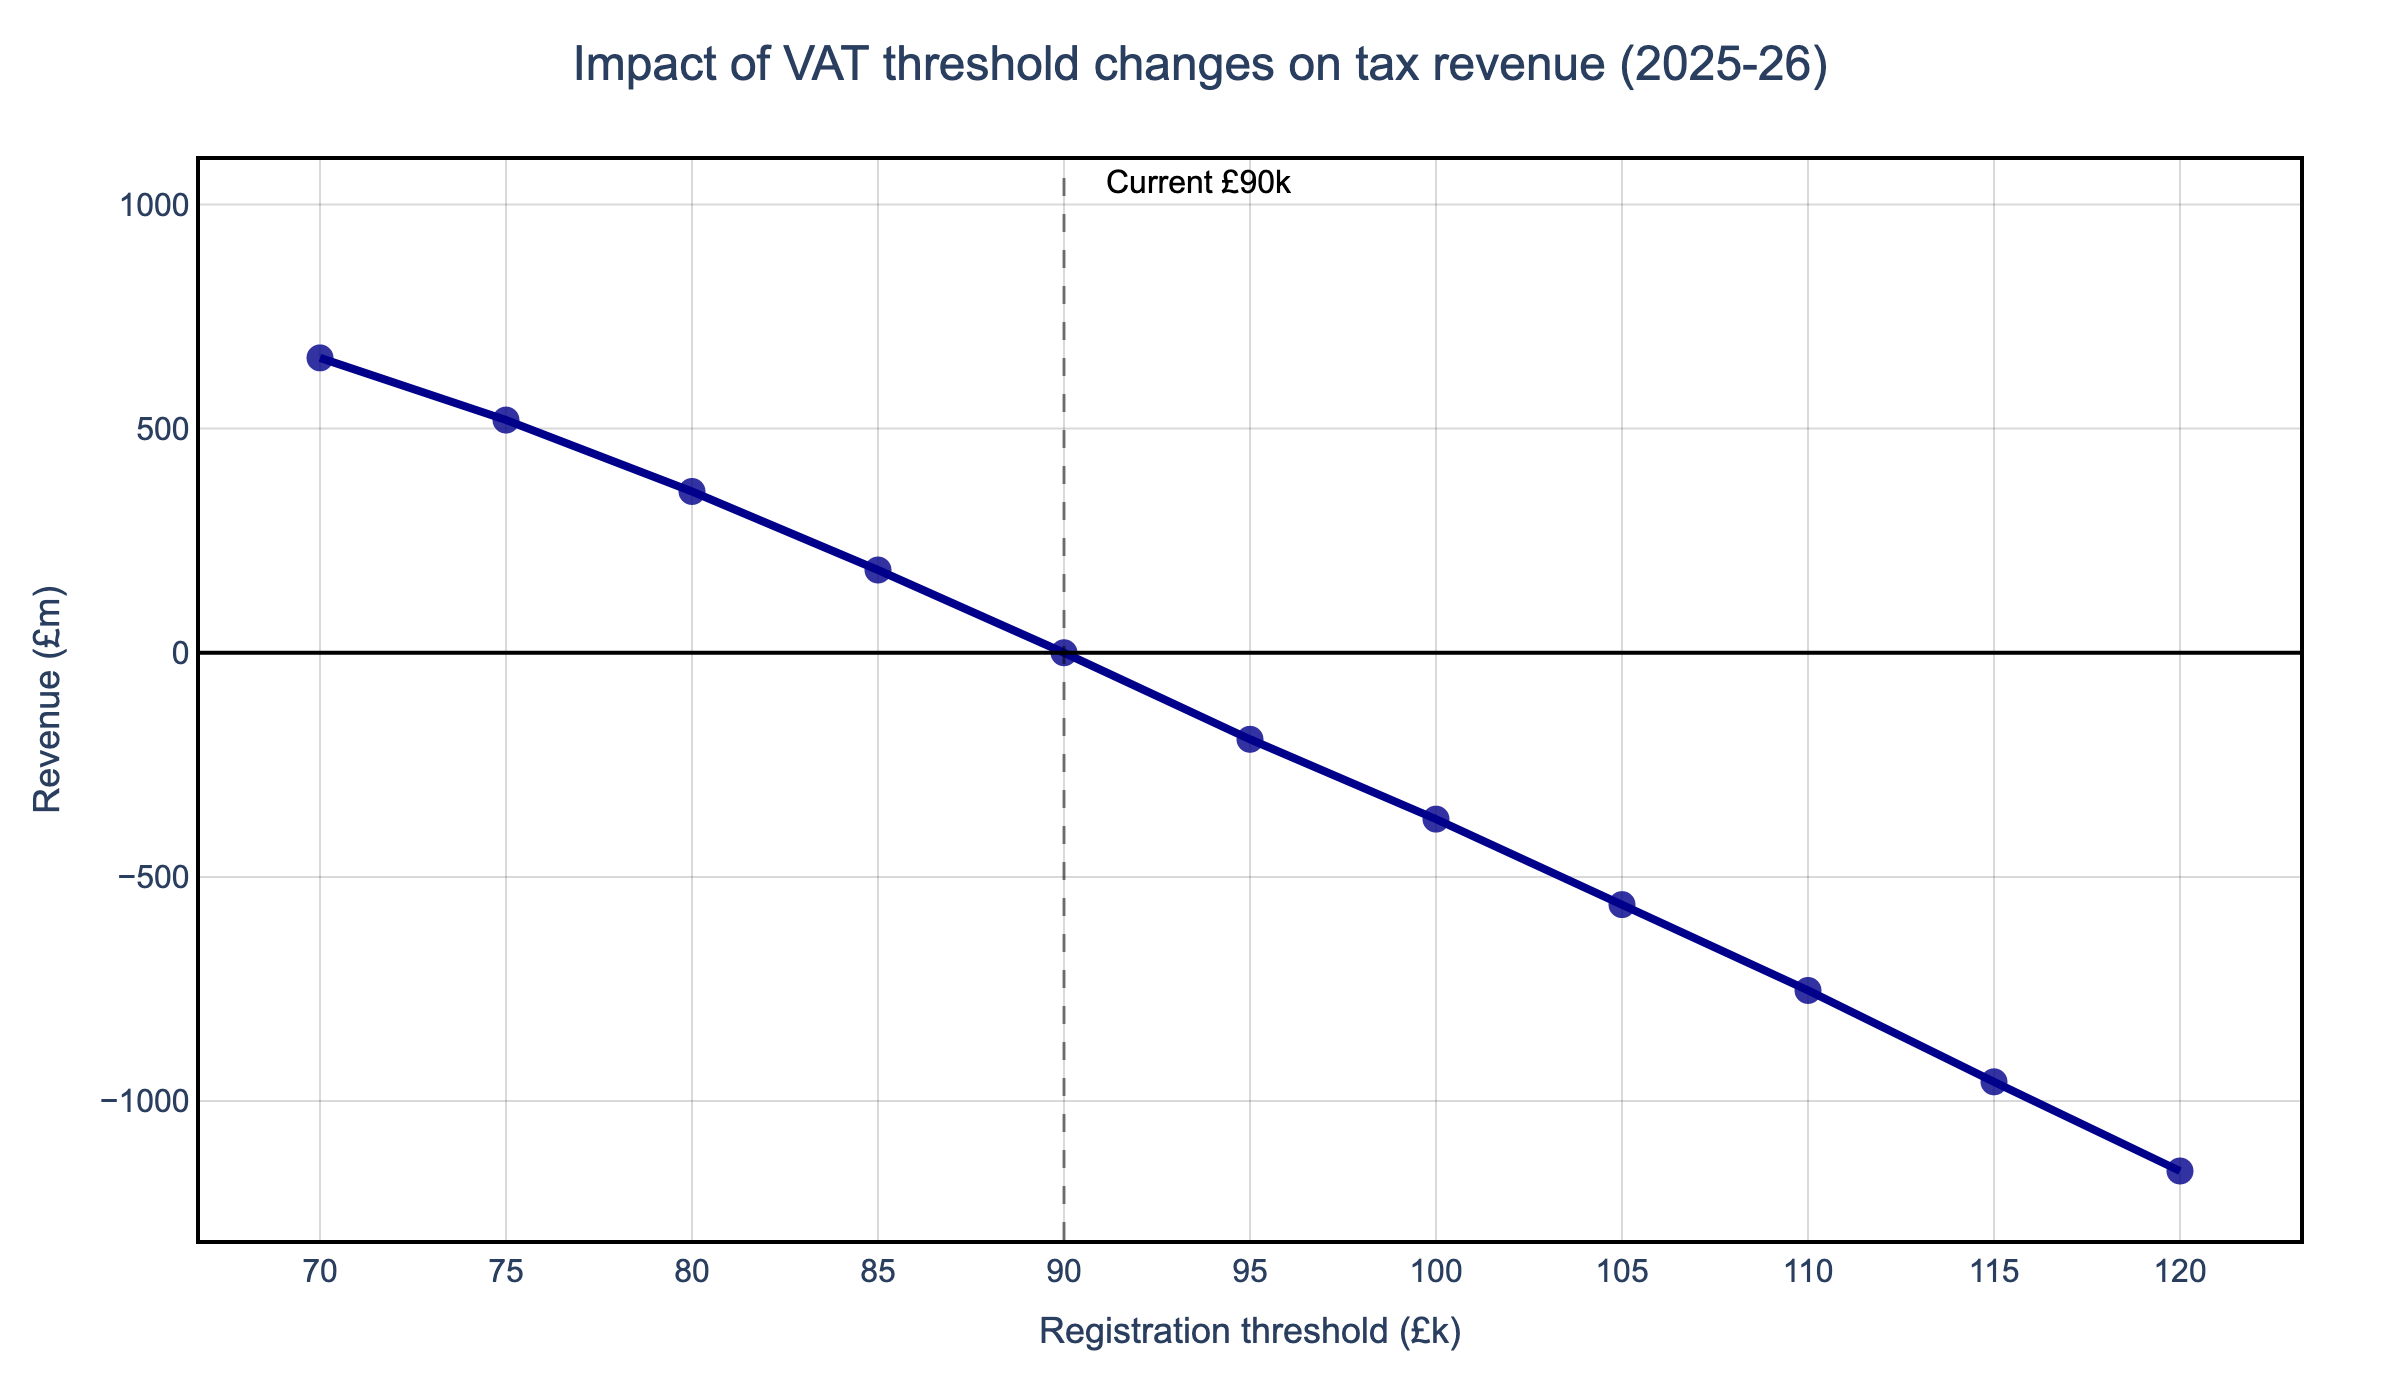
\includegraphics[width=0.85\textwidth]{figures/revenue_impact_2025_26.png}
\caption{Static revenue impact of changing the VAT registration threshold,
2025--26, relative to the \pounds90{,}000 baseline. Lowering the threshold raises
revenue; raising it loses revenue. The schedule is approximately linear over the
\pounds70{,}000--\pounds120{,}000 range.}
\label{fig:rev_impact}
\end{figure}

\begin{figure}[htbp]
\centering
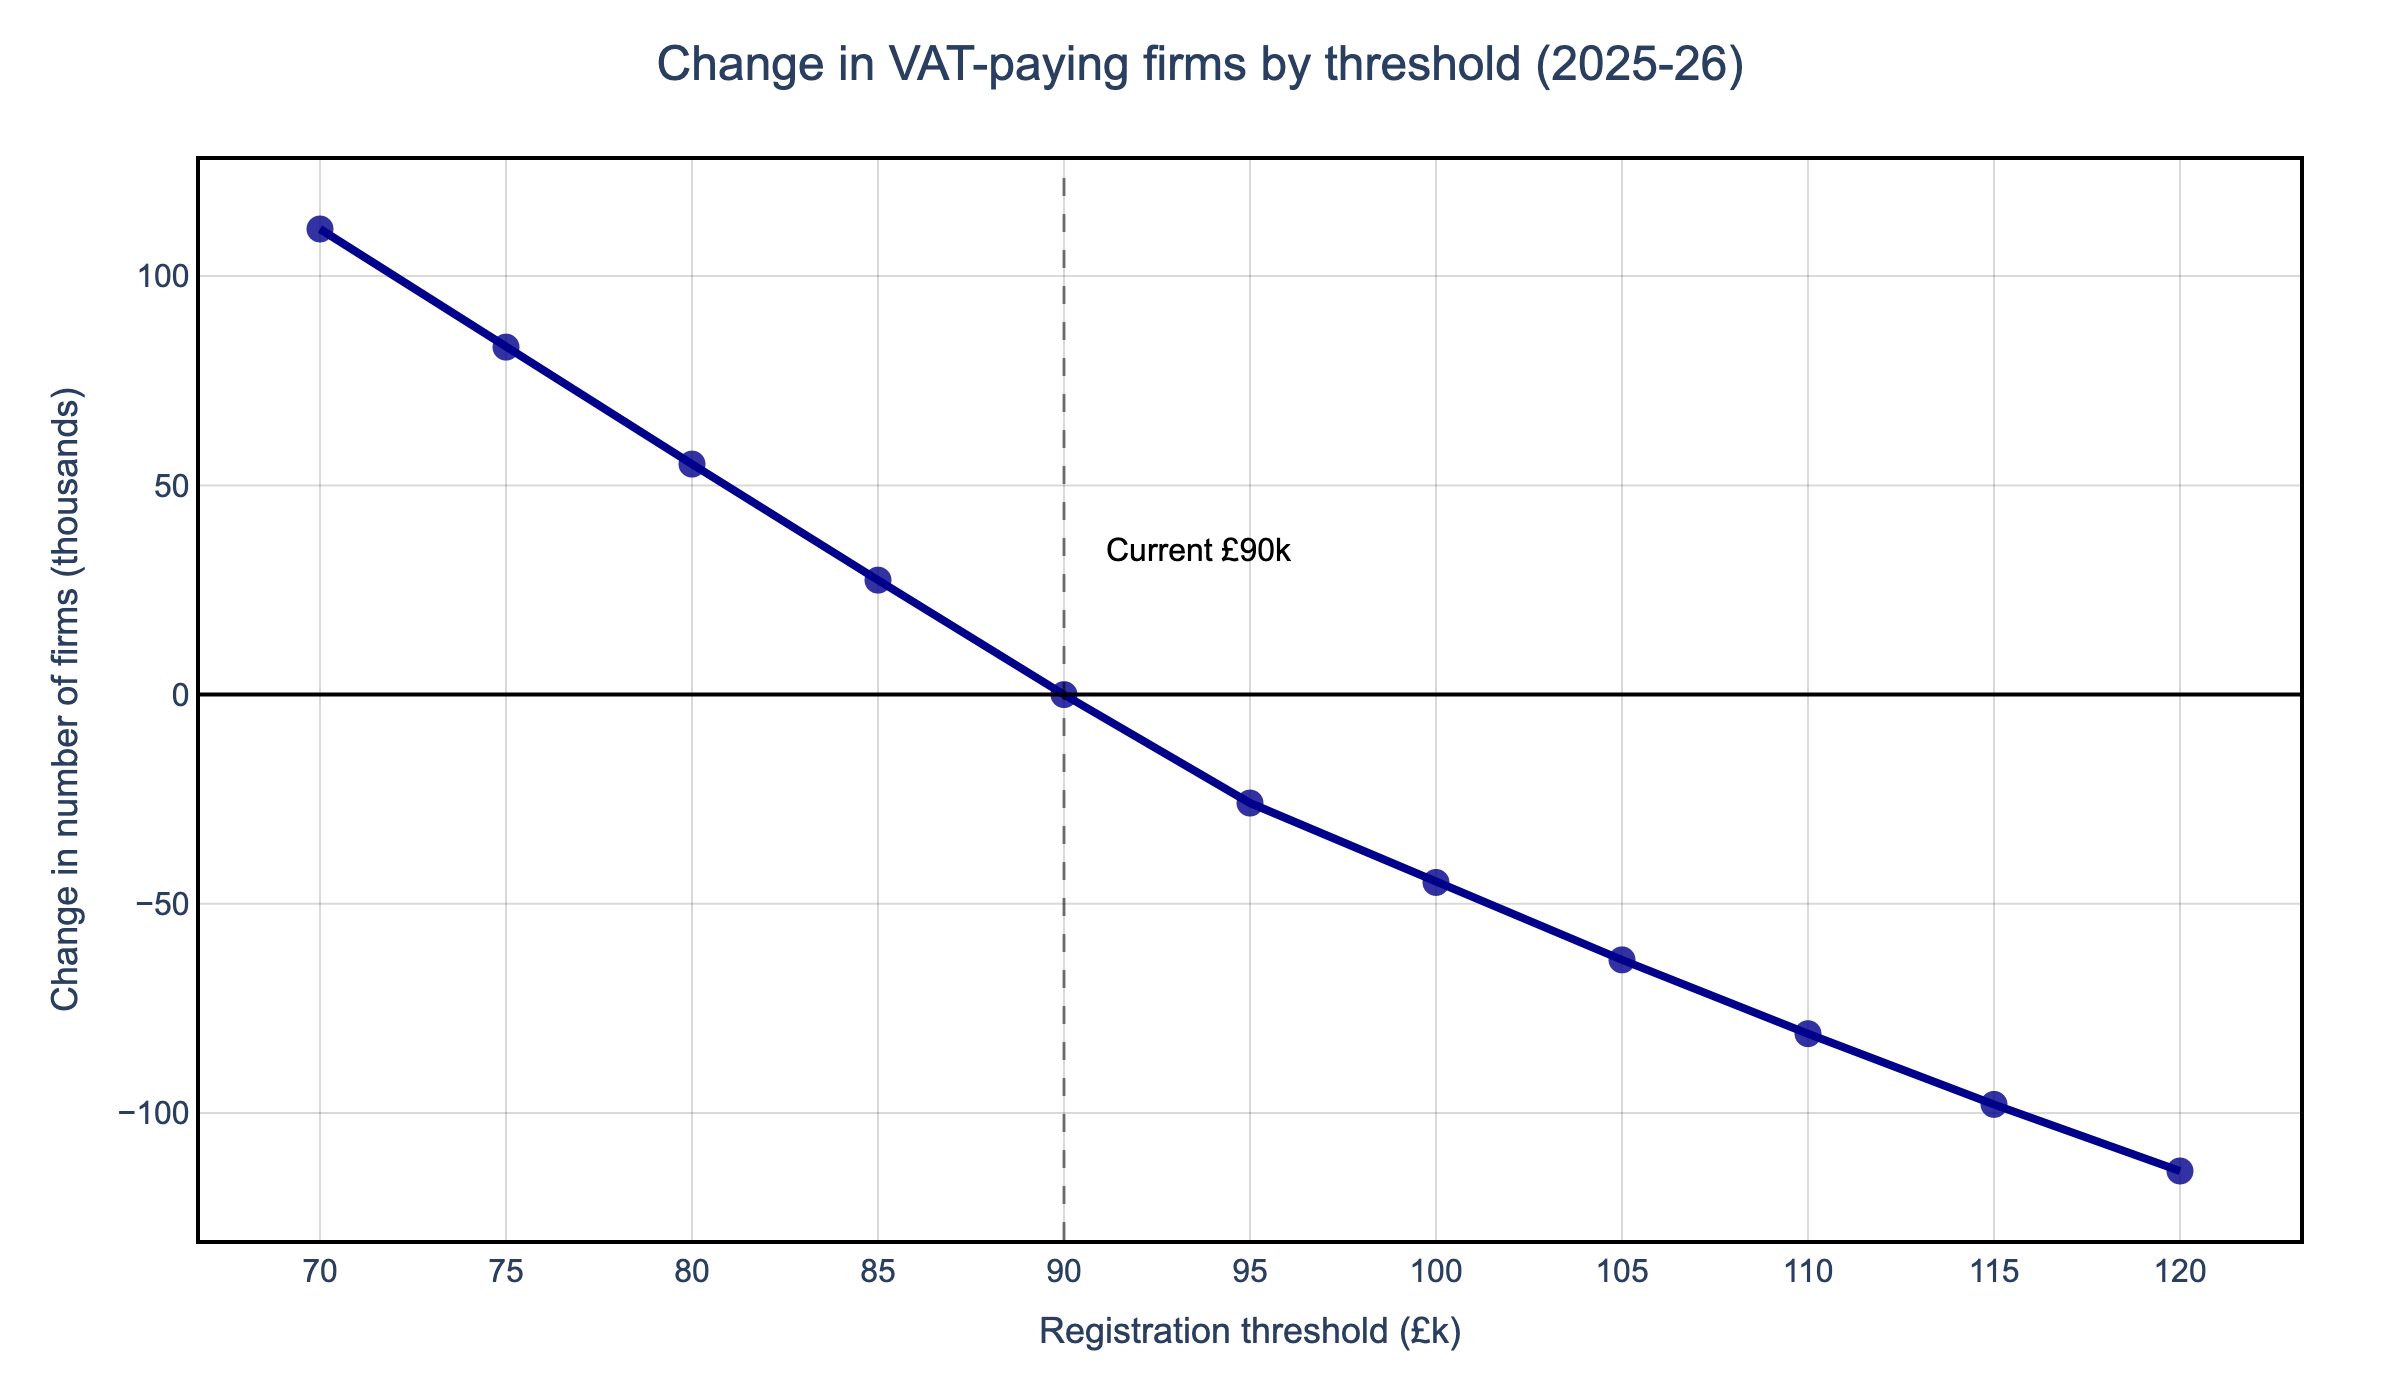
\includegraphics[width=0.85\textwidth]{figures/firms_impact_2025_26.png}
\caption{Number of firms affected by changing the VAT registration threshold,
2025--26, relative to the \pounds90{,}000 baseline. The count is roughly symmetric
around the baseline, tracking the local density of firms on each side of the
current threshold.}
\label{fig:firms_impact}
\end{figure}

\subsection{The behavioural response is modest and localised}
\label{sec:results_structural}

The static figures above assume firms do not respond to the changed schedule. The
calibrated model relaxes that assumption and quantifies how much firms actually
reposition; the central finding is that the realised response is small. The
headline behavioural object is the local turnover elasticity of
Section~\ref{sec:calibration} (median $\approx 0.17$), broadly in the range of the
UK VAT-base elasticity of \citet{liuetal2021}. The calibrated model is fitted to
reproduce the observed turnover distribution, so its close agreement with the data
(to within about $0.1\%$ on the bunching mass) is true by construction and I read
it only as an internal-consistency check, not a result. The informative contrast
is with the frictionless benchmark, and unlike the fit it is \emph{not}
mechanical: a Pure-FOC variant in which every firm re-optimises fully overstates
the response (Figure~\ref{fig:foc_dynamic}), implying a mean turnover of
\pounds1{,}488k against an actual \pounds1{,}130k.

Two regularities sharpen the interpretation. The response is \emph{partial}: only
about $15\%$ of near-threshold firms adjust, the rest held in place by
optimisation frictions and the discrete character of registration
\citep{chettyetal2011}. And it is \emph{localised}: firms that respond reposition
within roughly \pounds20{,}000 of the threshold. Realised behaviour at the notch
is therefore muted, so the aggregate behavioural offset to a threshold change is
small relative to the mechanical reclassification effect, and the static figures
of Table~\ref{tab:static_revenue} are a reasonable first approximation to the cost
of a threshold move.

\subsection{The graduated-taper reform}
\label{sec:results_taper}

I now report the schedule-shape reform of Section~\ref{sec:cf_taper}: replacing
the \pounds85{,}000 notch with a graduated taper whose effective rate phases
linearly from $0\%$ at \pounds85{,}000 to the full $20\%$ at \pounds105{,}000.
This is a counterfactual the reduced-form estimator cannot price, since a smooth
schedule leaves no single point of excess mass to forward-map; I re-solve each
firm's problem under the tapered schedule, holding the calibrated cost parameters
fixed, and compare with the model's \pounds85{,}000-notch baseline.

\paragraph{Efficiency case (analytic, robust).} The taper's case rests on an
exact, parameter-free property of the notch geometry. The \pounds85{,}000 notch
creates a \emph{dominated region} $(T^{*},\,T^{*}+a)=(\pounds85{,}000,\,
\pounds106{,}250)$ of width $a=T^{*}\tau_{\max}/(1-\tau_{\max})=\pounds21{,}250$
(Section~\ref{ssec:dominated}) that no firm optimally occupies---a pure
misallocation zone---together with a discrete drop of
$\tau_{\max}T^{*}\approx\pounds17{,}000$ in net revenue at the threshold. A
continuous taper has \emph{no} dominated region and \emph{no} discrete tax wedge:
marginal net revenue declines smoothly through the band rather than off a cliff,
so the discrete incentive to suppress turnover disappears. This follows
from~\eqref{eq:dominated} and the firm's problem~\eqref{eq:firm-problem}, with no
dependence on the smoothing parameter $k$, the returns-to-scale parameter
$\alpha$, or any simulated re-optimisation.

\paragraph{Revenue.} Against a baseline VAT base of \pounds179.3bn (the
\pounds85{,}000-notch year), the taper reduces revenue by \pounds335m on a
\emph{static} basis (firms in the band remit a tapered rather than a full rate,
turnover held fixed). I treat this static figure as the robust object. The
behavioural estimate---a larger loss of about \pounds889m once firms re-optimise
and expand into the low-rate band---is reported only as a directional indication:
it is sensitive to the smoothing parameter $k$ and the re-optimisation window and
I do not headline it. The reform affects about $227{,}000$ firms, of which
roughly $126{,}000$ ($125{,}608$ weighted) face a lower effective rate by sitting
in the \pounds85{,}000--\pounds105{,}000 band.

\paragraph{Sensitivity.} The revenue figures turn on the taper schedule and
turnover, not on the smoothed notch baseline, and are stable across $k$ and the
window. The \emph{simulated} change in near-threshold mass is not: the model's
notch-baseline bunching depends on $k$ (a steep $k$ concentrates a spike the taper
then cuts; at my calibrated $k=0.001$ the simulated notch barely bunches, so the
sign of the implied change reverses). I therefore rest the distributional
argument on the exact, $k$-free analytic mechanism above rather than on a
simulated magnitude.

\begin{figure}[htbp]
\centering
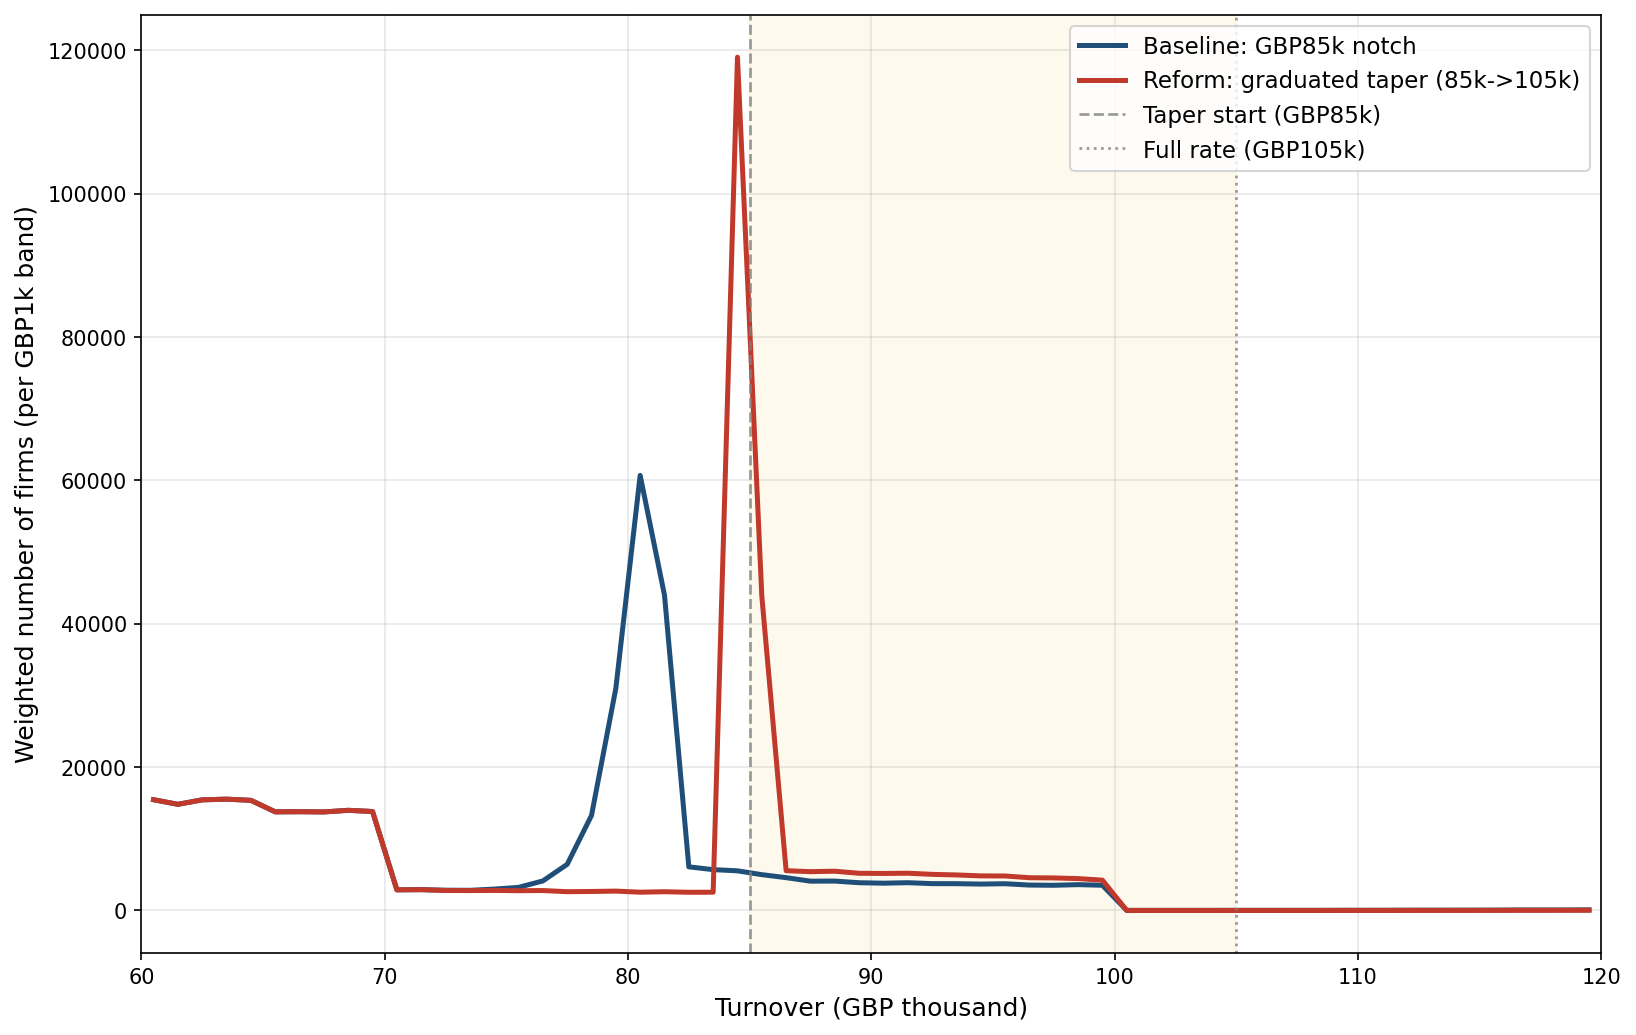
\includegraphics[width=0.9\textwidth]{figures/taper_reform_distribution.png}
\caption{Graduated-taper reform: firm-size distribution under the \pounds85{,}000
notch (baseline) versus the graduated taper that phases the effective VAT rate
linearly from $0\%$ at \pounds85{,}000 to $20\%$ at \pounds105{,}000 (shaded
band). The taper replaces the discrete notch---and its dominated region
$(\pounds85{,}000,\,\pounds106{,}250)$---with a smooth schedule, removing the
discrete incentive to suppress turnover. The precise simulated near-threshold mass
is sensitive to $k$ and the re-optimisation window, so I report the robust
revenue effect and the analytic efficiency mechanism rather than a distributional
magnitude.}
\label{fig:taper_reform}
\end{figure}

\subsection{A reduced rate for small firms}
\label{sec:results_rate}

The second schedule reform changes the \emph{rate} on a band: firms in the
\pounds85{,}000--\pounds105{,}000 band pay a reduced rate
$\tau_{\text{low}}\in\{10\%,15\%\}$ in place of the standard $20\%$, with $20\%$
retained above \pounds105{,}000. As with the taper, I re-solve each firm's
problem under the new banded schedule and compare with the \pounds85{,}000-notch
baseline.

\paragraph{Revenue.} Against the same \pounds179.3bn baseline, the banded reduced
rate reduces revenue, \emph{statically}, by \pounds357m at
$\tau_{\text{low}}=10\%$ and by \pounds178m at $\tau_{\text{low}}=15\%$, with
about $125{,}600$ firms in the band facing the lower rate. I report these static
figures as the robust object. The behavioural estimates are fragile to $k$ and the
window---the apparent behavioural \emph{gain} at $\tau_{\text{low}}=10\%$ (around
\(+\)\pounds723m) is an artefact of the bounded re-optimisation and the secondary
notch below, not a robust prediction---so I mention them only as directional.

\paragraph{Distortion case (analytic, robust).} The notch's discrete penalty
$\tau T^{*}$ and dominated region $a=T^{*}\tau/(1-\tau)$
(Section~\ref{ssec:dominated}) both shrink with the rate. At
$T^{*}=\pounds85{,}000$, lowering the rate from $20\%$ (penalty \pounds17{,}000,
region \pounds21{,}250) to $15\%$ cuts the region to \pounds15{,}000, and to
$10\%$ to \pounds9{,}444. A lower band rate mechanically shrinks the misallocation
zone, and with it the incentive to bunch.

\paragraph{Secondary notch.} The banded rate buys this at a cost the taper avoids:
because the rate steps back to $20\%$ at \pounds105{,}000, the reform introduces a
\emph{smaller secondary notch} at the band top (a step of
$20\%-\tau_{\text{low}}$ rather than the full $20\%$). The notch is attenuated and
relocated, not eliminated. The taper's continuous phase-in leaves no such step.

\paragraph{Scope: banded, not blanket.} I price only the \emph{banded}
small-firm reduced rate. A \emph{blanket} reduced rate on the whole registered
base is an economy-wide policy---of the order of \(-\)\pounds45bn at a $15\%$
standard rate and \(-\)\pounds90bn at $10\%$---whose incidence runs through
consumer pass-through and lies outside this partial firm model.

\subsection{Ranking the menu by efficiency}
\label{sec:results_efficiency}

The reforms cost broadly the same in static revenue (Table~\ref{tab:reform_menu}),
so the policy question is which buys the most distortion reduction per pound.
Table~\ref{tab:efficiency} ranks the menu on exactly that basis, and it is the
paper's central policy result.

The distortion measure is robust and analytic. The notch's dominated region
$(T^{*},\,T^{*}+a)$, $a=T^{*}\tau/(1-\tau)$, is a pure misallocation zone: no firm
optimally locates there, so its width is a clean, $k$-free,
$\alpha$-free index of the discrete distortion the notch imposes. For each reform
I ask how much of this zone it removes. Raising the threshold to \pounds100{,}000
simply \emph{relocates} the same \pounds21{,}250 zone to the new cutoff, removing
essentially none of it at a static cost of \pounds371m. A reduced rate
\emph{shrinks} the zone: to \pounds15{,}000 at $15\%$ (removing \pounds6{,}250)
and to \pounds9{,}444 at $10\%$ (removing \pounds11{,}806). The graduated taper
\emph{eliminates} it: a continuous schedule has no dominated region, so the whole
\pounds21{,}250 zone is removed---and at a static cost (\pounds335m) below that of
the threshold move.

\begin{table}[htbp]
\centering
\caption{Reform-menu comparison: static, behaviour-free revenue effect of the four
reforms at comparable scale, relative to the \pounds85{,}000-notch baseline (VAT
base \pounds179.3bn for the schedule reforms; the threshold move is measured
against the post-reform \pounds90{,}000 baseline of
Table~\ref{tab:static_revenue}). Each reform pulls a different lever---location,
schedule shape, or rate. Figures are static; behavioural estimates are reported
and caveated as directional in the relevant subsections.}
\label{tab:reform_menu}
\begin{tabular}{llr}
\toprule
Reform & Lever & Static revenue (\pounds m) \\
\midrule
Raise threshold to \pounds100{,}000 & Location & $-371$ \\
Graduated taper $[\pounds85\text{k},\pounds105\text{k}]$ & Shape (phase-in) & $-335$ \\
Reduced rate $10\%$ $[\pounds85\text{k},\pounds105\text{k}]$ & Rate (step) & $-357$ \\
Reduced rate $15\%$ $[\pounds85\text{k},\pounds105\text{k}]$ & Rate (step) & $-178$ \\
\bottomrule
\end{tabular}
\end{table}

\begin{table}[htbp]
\centering
\caption{Efficiency ranking of the reform menu. The dominated region
$(T^{*},\,T^{*}+a)$, $a=T^{*}\tau/(1-\tau)$ (Section~\ref{ssec:dominated}), is a
pure misallocation zone of width \pounds21{,}250 under the current
\pounds85{,}000/$20\%$ notch. ``Distortion removed'' is the reduction in the width
of this zone; static revenue is from Table~\ref{tab:reform_menu}. This is a
robust, analytic deadweight/misallocation comparison based on the dominated
region, \emph{not} a full welfare integral (which would require value added and
input reclaim; see Section~\ref{sec:conclusion}). Reforms are ordered from least
to most distortion removed.}
\label{tab:efficiency}
\begin{tabular}{llrrr}
\toprule
Reform & Lever & Static rev. (\pounds m) & Dominated region & Distortion removed \\
\midrule
Raise threshold to \pounds100{,}000 & Location & $-371$ & \pounds21{,}250 (relocated) & $\approx\pounds0$ \\
Reduced rate $15\%$ & Rate & $-178$ & \pounds15{,}000 & \pounds6{,}250 \\
Reduced rate $10\%$ & Rate & $-357$ & \pounds9{,}444 & \pounds11{,}806 \\
Graduated taper & Shape & $-335$ & \pounds0 (no notch) & \pounds21{,}250 (whole zone) \\
\bottomrule
\end{tabular}
\end{table}

The ranking carries a clear message: \emph{schedule reforms dominate
threshold-location moves on efficiency}. A location move is fiscally comparable to
the schedule reforms but buys almost no distortion reduction---it merely transports
the misallocation zone to a new threshold. The reduced rate shrinks the zone, more
so the lower the rate. The graduated taper is the efficiency winner: it removes the
entire misallocation zone, and does so at a lower static cost than raising the
threshold. The reduced rate sits between the two on the same frontier, simpler than
the taper but reintroducing a smaller secondary notch at the band top that the
taper's continuous phase-in avoids.

The cross-check in Table~\ref{tab:reform_menu} is reassuring: the flat-$10\%$ band
(\(-\)\pounds357m) costs almost exactly what the taper costs
(\(-\)\pounds335m), because a $0\%\to20\%$ linear phase-in averages roughly $10\%$
over the band, so two differently-shaped schedules impose nearly the same average
burden. I label the efficiency comparison honestly: it is a
deadweight/misallocation ranking based on the dominated-region distortion, which is
robust and analytic, not a full welfare integral. Converting these distortion
measures into welfare or MVPF terms requires modelling value added and input
reclaim and is left to future work (Section~\ref{sec:conclusion}).
